
\section{Graphen}

\subsection{BCC-Gitter}

\begin{figure}[H]
\begin{minipage}[b]{0.3\textwidth}
    \centering
    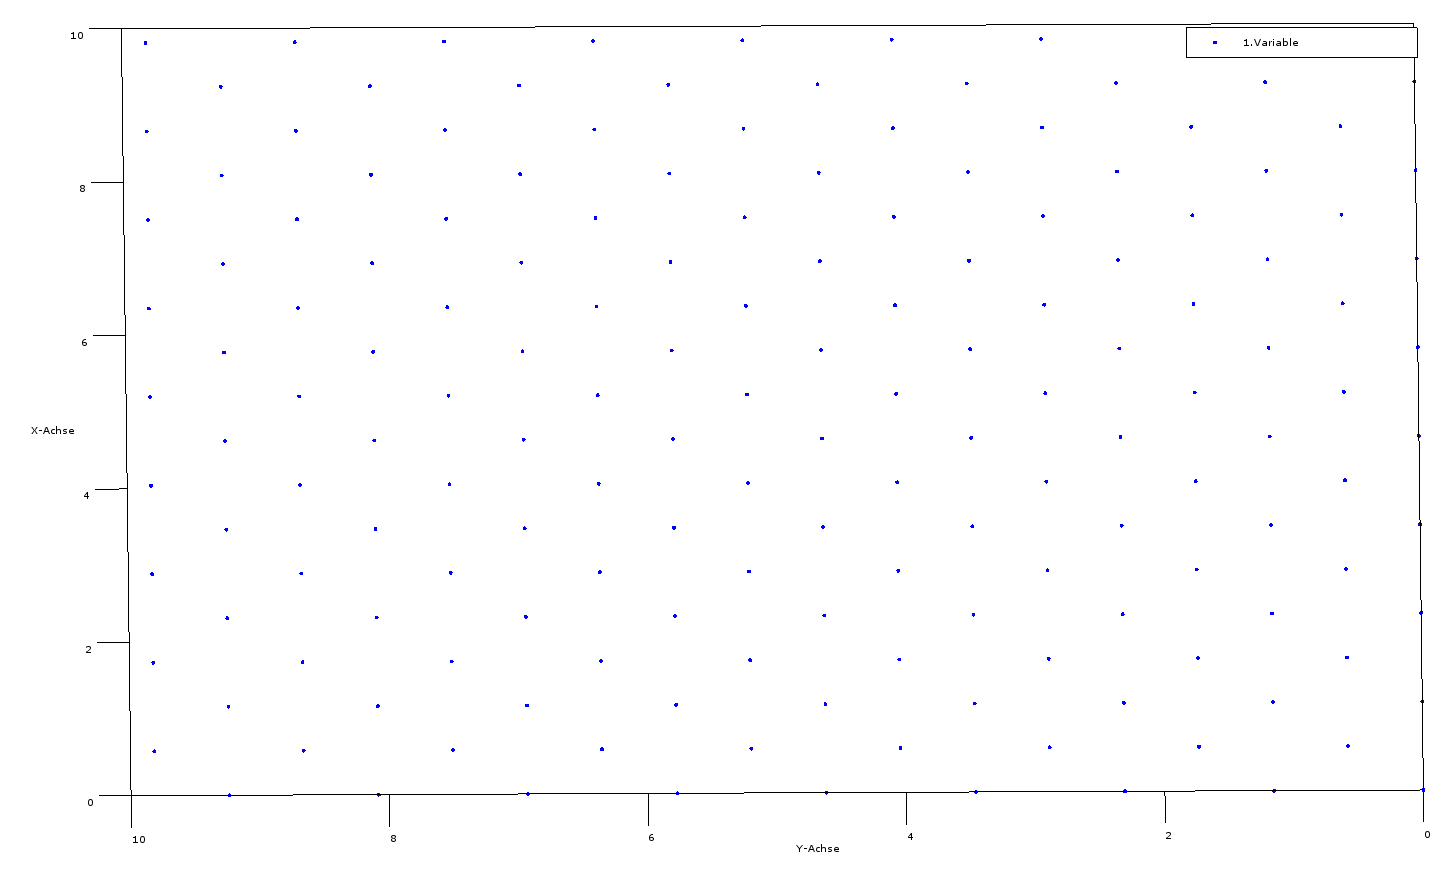
\includegraphics[scale=0.12]{data/bcc_x-y.PNG}
    \caption{BCC: xy-Ebene}
    \label{fig:bccxy}
\end{minipage}    
\begin{minipage}[b]{0.3\textwidth}
    \centering
    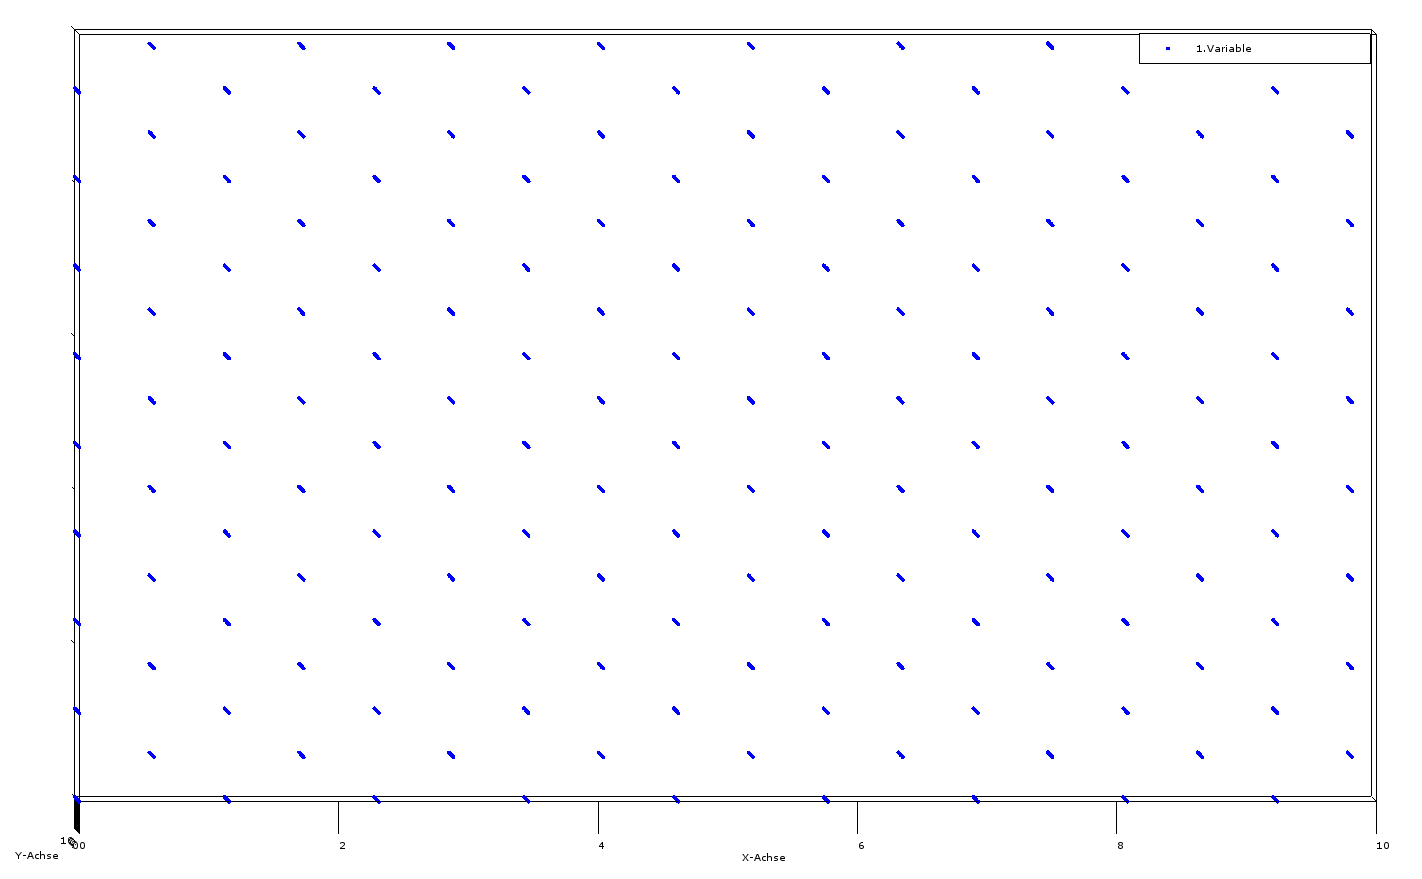
\includegraphics[scale=0.12]{data/bcc_x-z.PNG}
    \caption{BCC: xz-Ebene}
    \label{fig:bccxz}
\end{minipage} 
\begin{minipage}[b]{0.3\textwidth}
    \centering
    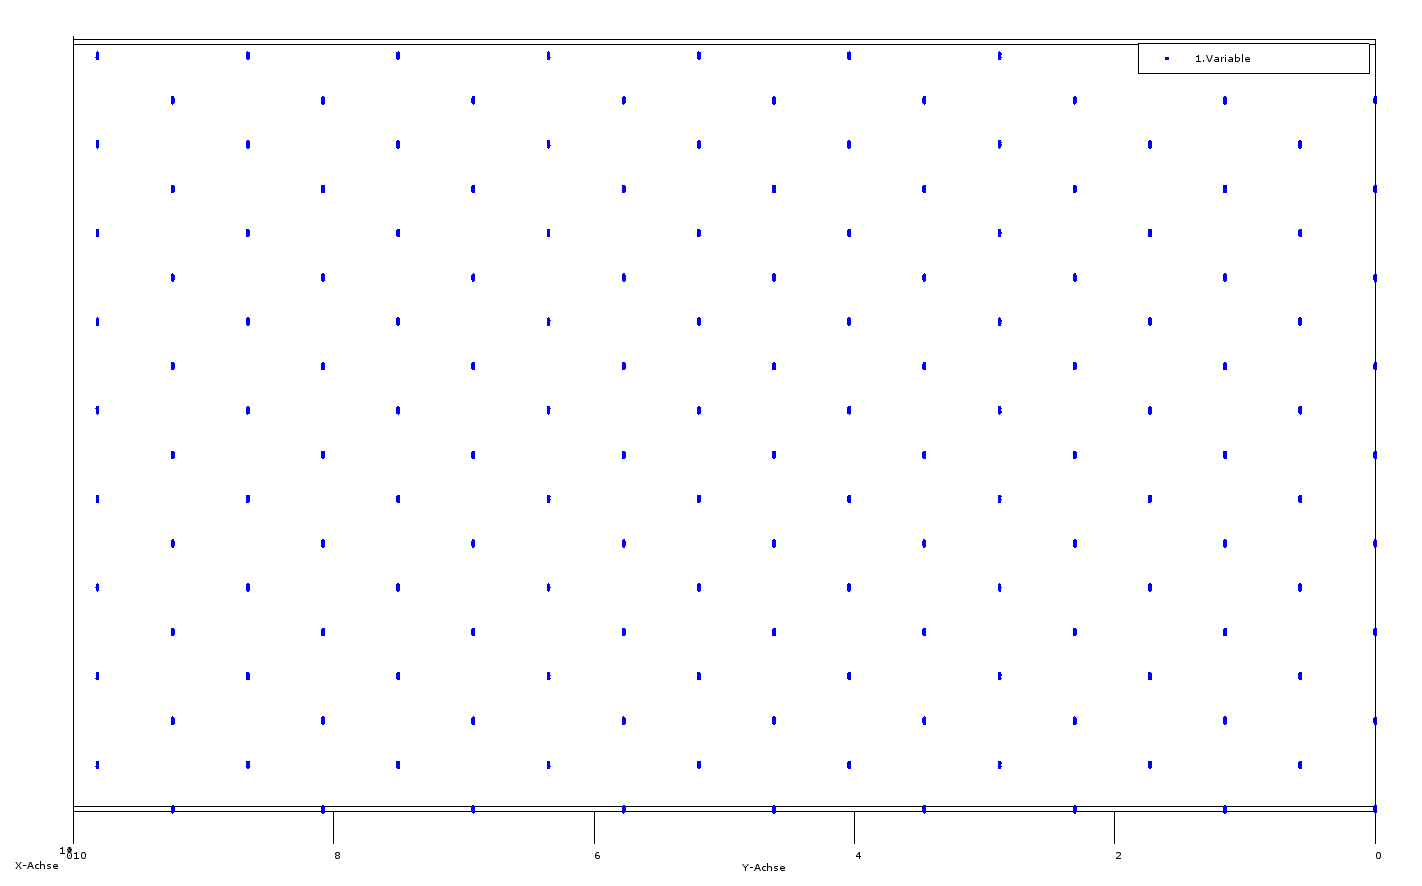
\includegraphics[scale=0.12]{data/bcc_y-z.PNG}
    \caption{BCC: yz-Ebene}
    \label{fig:bccyz}
\end{minipage} 
\end{figure}

\begin{figure}[H]
\begin{minipage}[b]{0.5\textwidth}
    \centering
    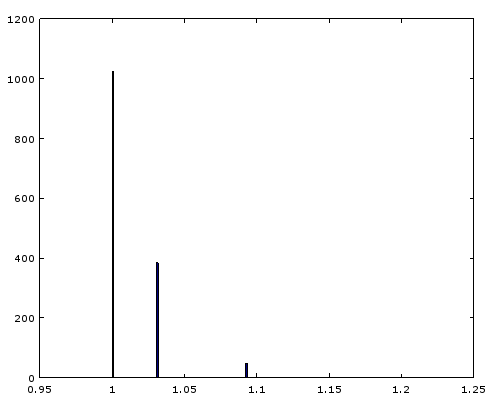
\includegraphics[scale=0.5]{data/bcc-hist.PNG}
    \caption{BCC: Teilchenabstände}
    \label{fig:bccabstand}
\end{minipage}    
\begin{minipage}[b]{0.5\textwidth}
    \centering
    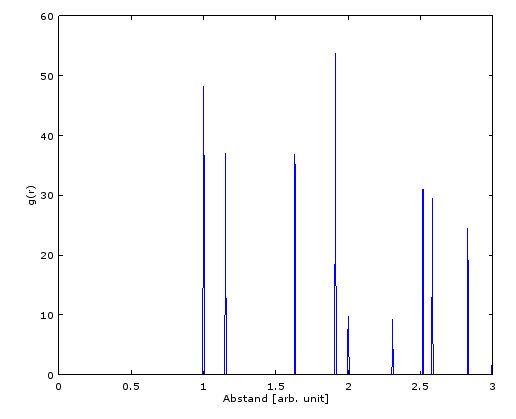
\includegraphics[scale=0.5]{data/bcc-paircorrelation.PNG}
    \caption{BCC: Paarkorrelationsfunktion}
    \label{fig:bccg}
\end{minipage} 
\end{figure}

\subsection{FCC-Gitter}

\begin{figure}[H]
\begin{minipage}[b]{0.3\textwidth}
    \centering
    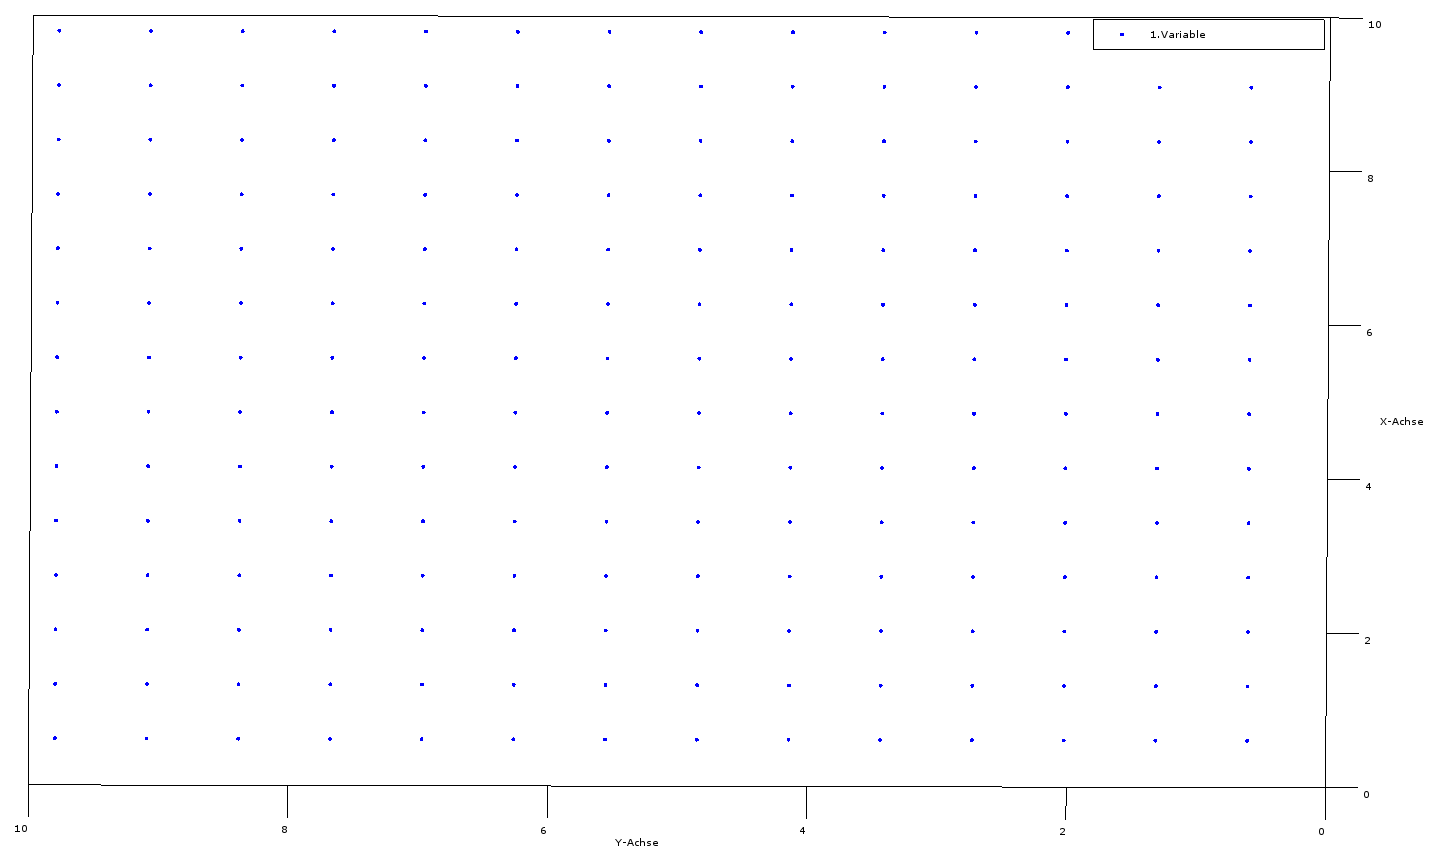
\includegraphics[scale=0.12]{data/fcc_x-y.PNG}
    \caption{FCC: xy-Ebene}
    \label{fig:fccxy}
\end{minipage}    
\begin{minipage}[b]{0.3\textwidth}
    \centering
    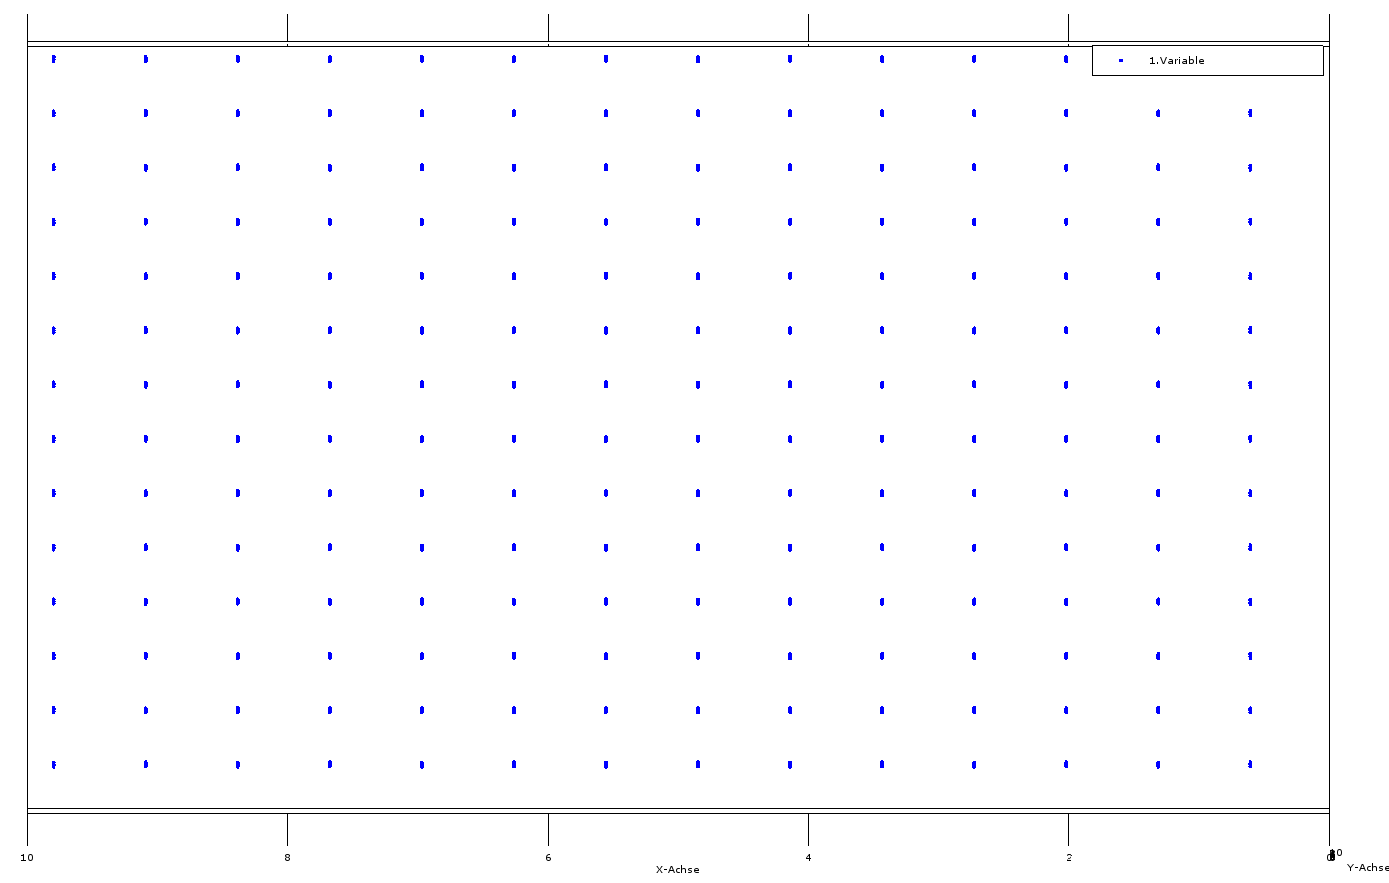
\includegraphics[scale=0.12]{data/fcc_x-z.PNG}
    \caption{FCC: xz-Ebene}
    \label{fig:fccxz}
\end{minipage} 
\begin{minipage}[b]{0.3\textwidth}
    \centering
    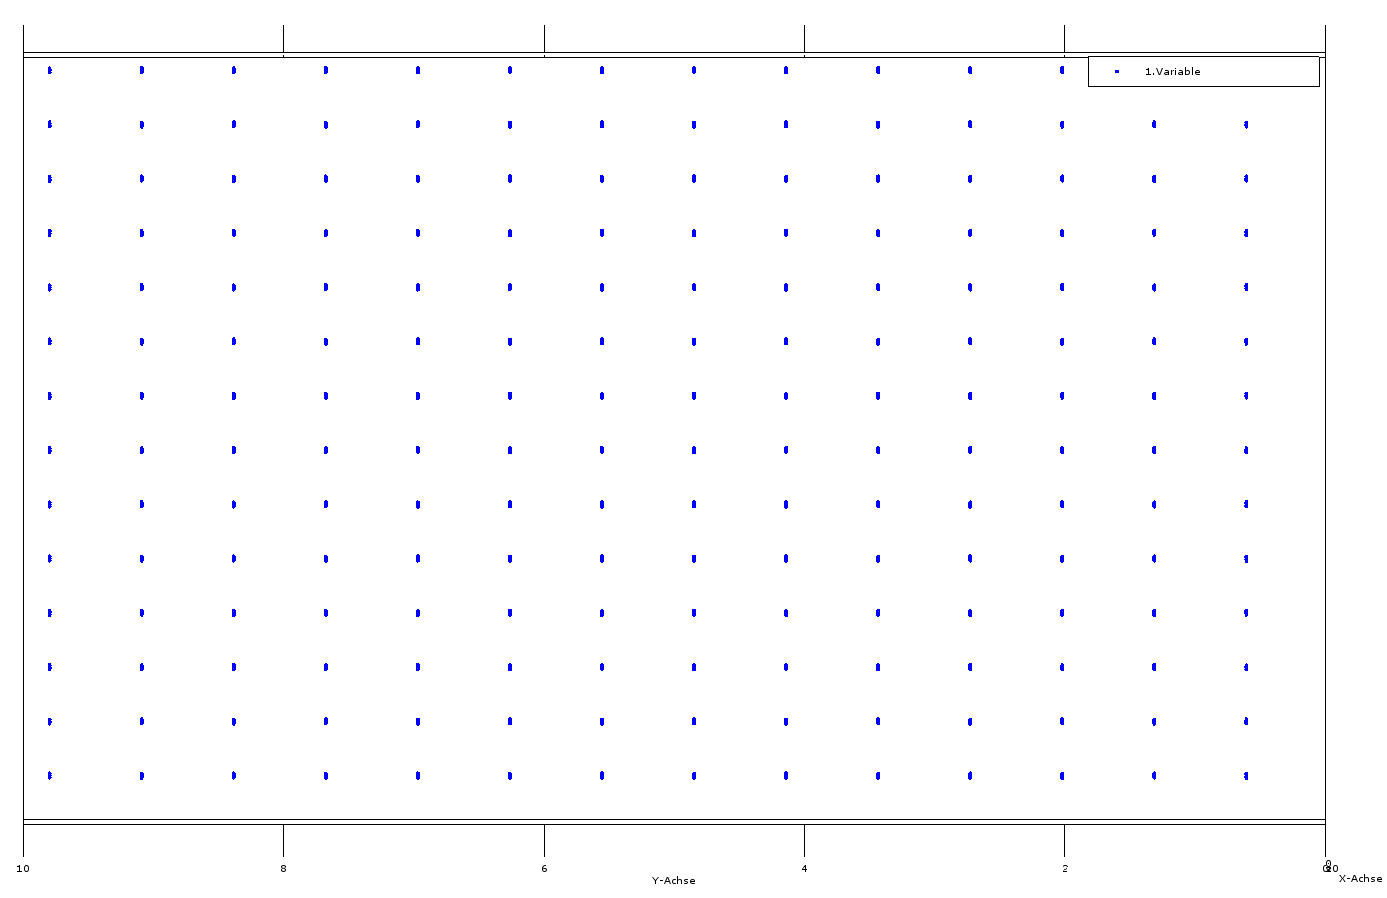
\includegraphics[scale=0.12]{data/fcc_y-z.PNG}
    \caption{FCC: yz-Ebene}
    \label{fig:fccyz}
\end{minipage} 
\end{figure}

\begin{figure}[H]
\begin{minipage}[b]{0.5\textwidth}
    \centering
    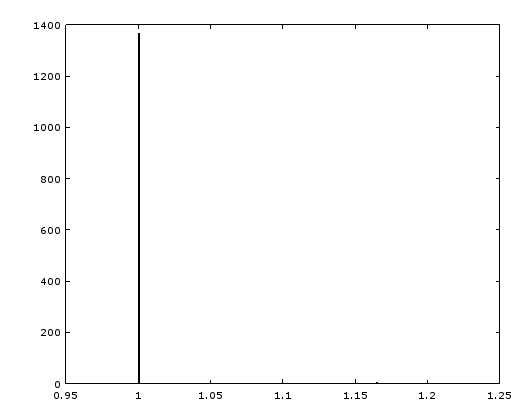
\includegraphics[scale=0.5]{data/fcc-hist.PNG}
    \caption{FCC: Teilchenabstände}
    \label{fig:fccabstand}
\end{minipage}    
\begin{minipage}[b]{0.5\textwidth}
    \centering
    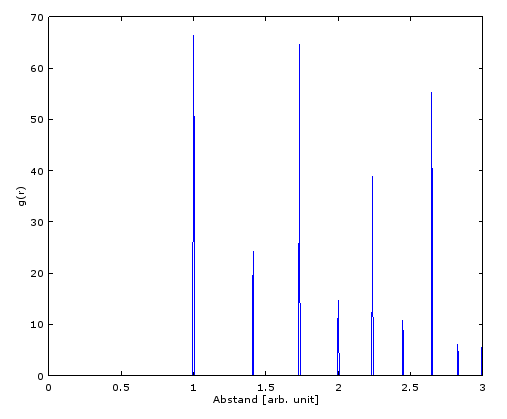
\includegraphics[scale=0.5]{data/fcc-paircorrelation.PNG}
    \caption{FCC: Paarkorrelationsfunktion}
    \label{fig:fccg}
\end{minipage} 
\end{figure}

\subsection{HCP-Gitter}

\begin{figure}[H]
\begin{minipage}[b]{0.3\textwidth}
    \centering
    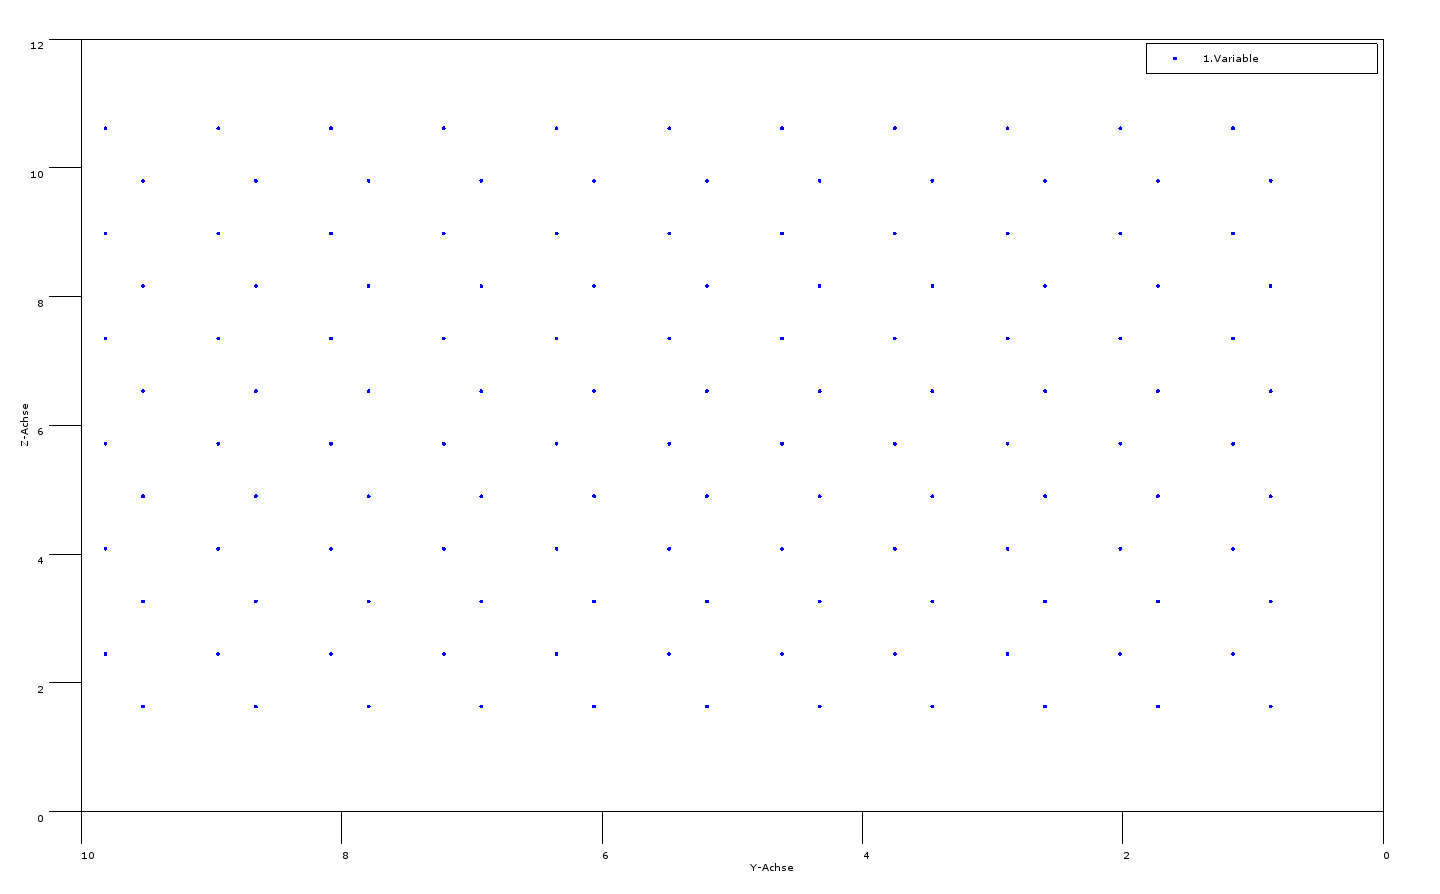
\includegraphics[scale=0.12]{data/hcp_x-y.PNG}
    \caption{HCP: xy-Ebene}
    \label{fig:hcpxy}
\end{minipage}    
\begin{minipage}[b]{0.3\textwidth}
    \centering
    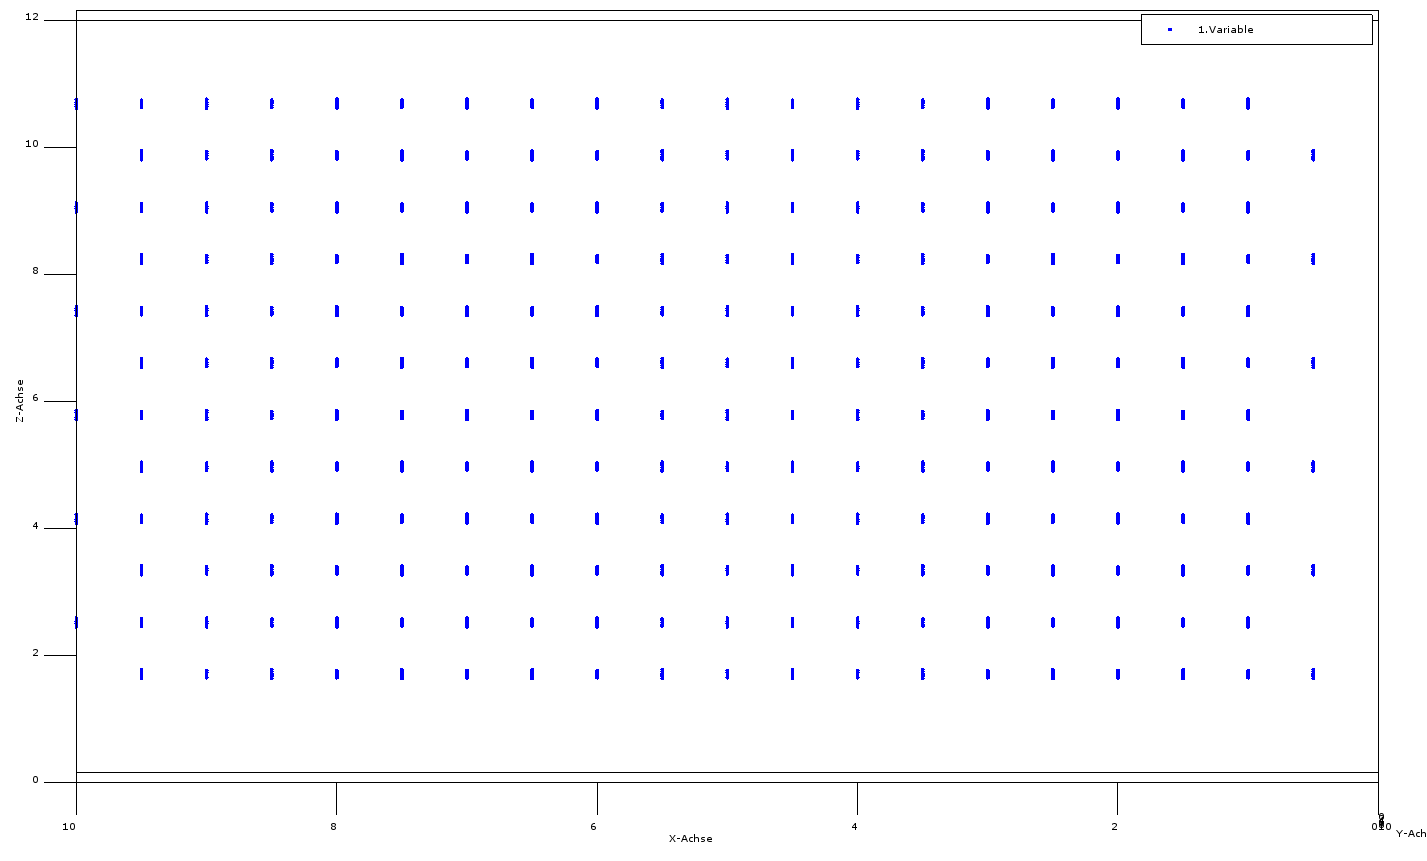
\includegraphics[scale=0.12]{data/hcp_z-x.PNG}
    \caption{HCP: xz-Ebene}
    \label{fig:hcpxz}
\end{minipage} 
\begin{minipage}[b]{0.3\textwidth}
    \centering
    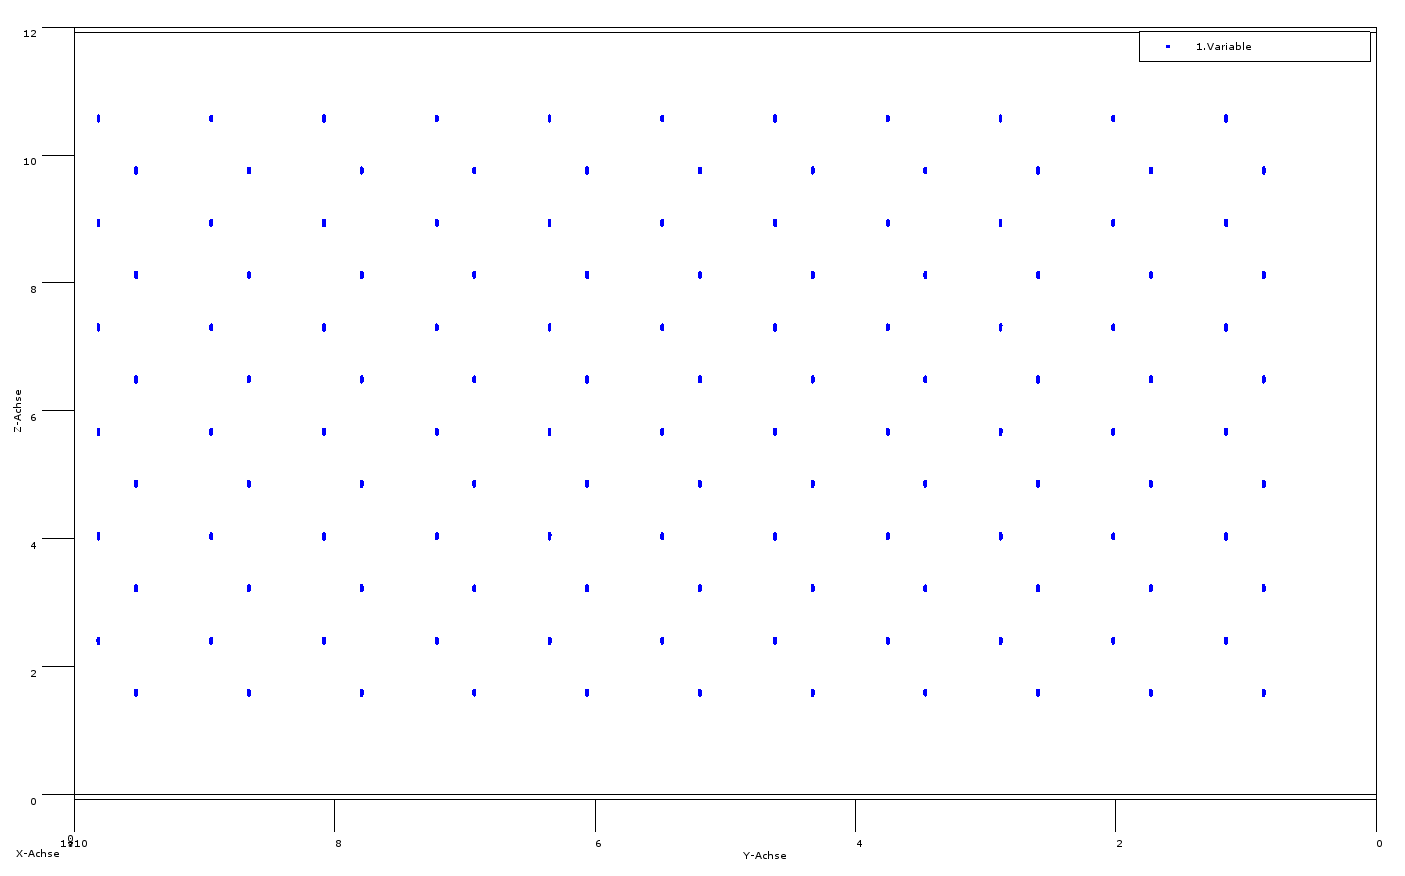
\includegraphics[scale=0.12]{data/hcp_z-y.PNG}
    \caption{HCP: yz-Ebene}
    \label{fig:hcpyz}
\end{minipage} 
\end{figure}

\begin{figure}[H]
\begin{minipage}[b]{0.5\textwidth}
    \centering
    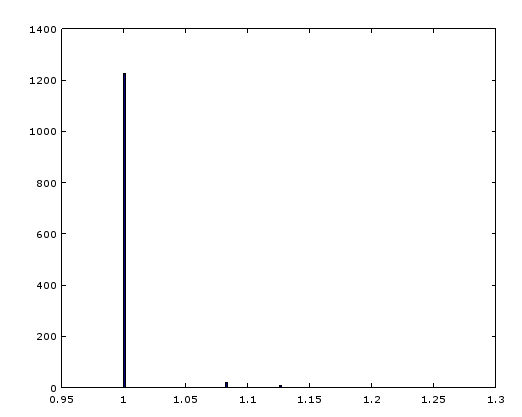
\includegraphics[scale=0.5]{data/hcp-hist.PNG}
    \caption{HCP: Teilchenabstände}
    \label{fig:hcpabstand}
\end{minipage}    
\begin{minipage}[b]{0.5\textwidth}
    \centering
    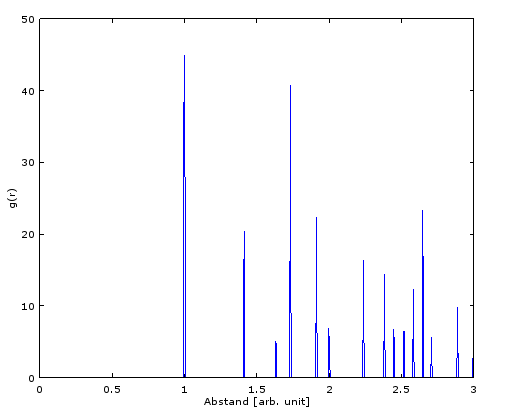
\includegraphics[scale=0.5]{data/hcp-paircorrelation.PNG}
    \caption{HCP: Paarkorrelationsfunktion}
    \label{fig:hcpg}
\end{minipage} 
\end{figure}










\FloatBarrier
\pagebreak
\newpage
\begin{landscape}
\section{Messwerte}

\begin{table}[H]
\begin{tabular}{|l|llll|l|l|}
    \multicolumn{7}{l}{Horizontale Abstände}\\ \hline
     &Mitte – unten &Mitte - halbe Höhe &Halber Radius – unten &halber Radius - halbe Höhe & &\\ \hline
     &6.75 &8 &8.36 &8.5016 & &\\
     &7.125 &8.75 &8.2971 &9.2525 & &\\
     &7.6833 &9.75 &8.4 &9.208 &Mittelwert: &Anzahl:\\\hline
    Mittelwerte: &7.19 &8.83 &8.35 &8.99 &8.34 &192.57894\\\hline
    \multicolumn{7}{l}{}\\
    \multicolumn{7}{l}{Vertikale Abstände}\\ \hline
     &6.3433 &6.8333 &6.4 &6.604 & &\\
     &6.6 &6.2 &5.2 &7.2 & &\\
     &5.25 &5.8333 &5.75 &7.755 &Mittelwert: &Anzahl:\\\hline
    Mittelwerte: &6.06 &6.29 &5.78 &7.19 &6.33 &146.16603\\\hline
\end{tabular}
\caption{Messwerte zur Anzahlbestimmung}
\label{tab:mess-anz}
\end{table}

\begin{table}[H]
\begin{tabular}{|l|l|l|} \hline
Horizontale Weite in mm ???& Horizontale Anzahl & Anzahl Grundfläche \\
1409 & 168.94 & 22415.83 \\ \hline
vertikale Weite in mm ???& vertikale Anzahl & Anzahl Volumen \\ 
120 & 18.96 & \cellcolor[HTML]{C0C0C0}{\color[HTML]{FD6864} 425004} \\ \hline
\end{tabular}
\caption{Anzahlbestimmung}
\label{tab:anz}
\end{table}
\end{landscape}

\pagebreak
